
\section{Ejercicio 1: Reducción de dimensiones}

\subsection{Introducción}

\par Para el primer ejercicio, queremos reducir la dimensionalidad de la entrada, debido a que es muy grande, a 3 valores. Para esto vamos a diseñar una red neuronal y la entrenaremos mediante aprendizaje hebbiano no supervisado aplicando la regla de oja y la regla de sanger. Luego analizaremos y compararemos sus resultados.

\subsection{Análisis de la Red}

\par En un comienzo, trabajamos con una red que contaba con 10 o 15 neuronas de salida para no reducir drásticamente su dimensión. Al final el entrenamiento, reducíamos la salida a 3 valores y obteníamos lo buscado. Luego de varias pruebas y cambios determinamos que no ganábamos nada tomando esta determinación, por el contrario, se áumentaba la complejidad del algoritmo y se perdía tiempo revisando la ortogonalidad de las 10 columnas de la matriz de pesos, mientras que los resultados obtenidos no eran mejores. Por esto se determinó manejar desde un inicio 3 dimensiones de salida.

\par Vale aclarar que las reglas de oja y sanger son formas de calcular el cambio que se debe hacer a la matriz de pesos para entrenarla. Por esto, ambos modelos son iguales, solo que se aplican distintos cálculos para cada tipo de regla.

\subsection{Procesamiento de Datos}

\par Sabemos que los valores de entrada son enteros positivos, ya que determinan la cantidad de apariciones de una palabra en un texto. Y al estar la entrada preprocesada y sin las palabras mas comunes (con mas apariciones), los valores de entrada se encuentran acotados. Podríamos no haber implementado ningún tipo de preprocesamiento, pero preferimos estandarizar la entrada, de manera que los atributos presenten media cero y varianza uno, moviendose en un rango de valores similar.


\subsection{Experimentación y Resultados}

\par Habiendo fijado el número de neuronas de salida a tres unidades, pasamos a implementar los dos algoritmos propuestos. En primera instancia trabajamos en una fase de entrenamiento, donde el parámetro de interés a optimizar es el coeficiente de aprendizaje, que bien puede ser función del número de época. Tanto la condición de ortonormalidad( $|| W^T \cdot W - I || = 0$) como la subsiguiente validación son las herramientas para determinar su valor óptimo. Comenzamos con un coeficiente de aprendizaje constante, siguiendo con funciones del tipo $\frac{1}{epoca^{\alpha}}$, con alfa entre 0 y 1. Probando estas distintas opciones encontramos que si bien no existían diferencias significativas, un coeficiente del tipo $\frac{1}{epoca^{\frac{1}{2}}}$ presentaba los mejores resultados.

\subsubsection{Algoritmo de Oja}

\par A continuación se pueden observar los resultados obtenidos utilizando el algoritmo de Oja separando el set de datos de entrada en 70\% - 30\%, para el coeficiente de aprendizaje adaptativo propuesto. Las figuras \ref{fig:  ej1_oja_3d_1} y \ref{fig: ej1_oja_3d_2} presentan los datos en el espacio 3d de salida obtenido por el algoritmo. Las figuras \ref{fig: ej1_oja_3d_1_train} y \ref{fig: ej1_oja_3d_2_train} corresponden a datos de entrenamiento, mientras que las figuras \ref{fig: ej1_oja_3d_1_valid} y \ref{fig: ej1_oja_3d_2_valid} corresponden a datos de validación. 

\begin{figure}[H]
        \begin{subfigure}[b]{0.5\textwidth}
                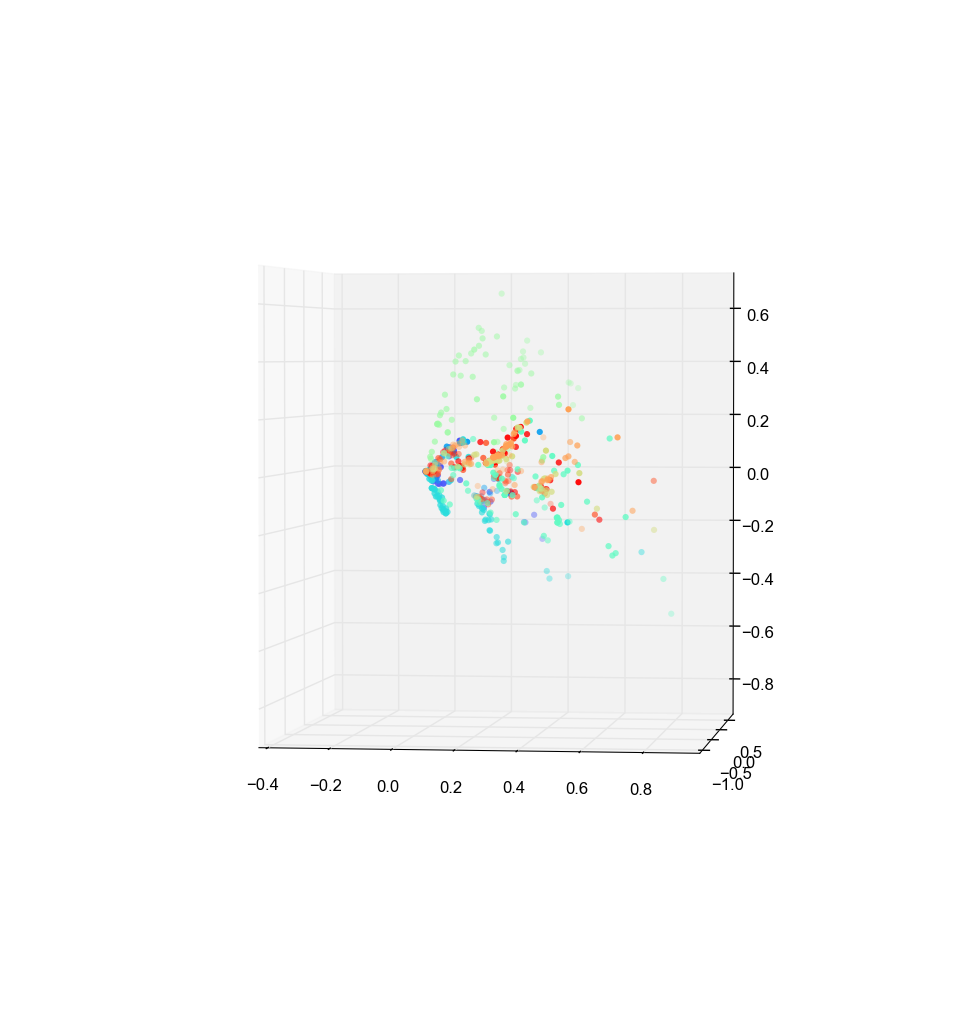
\includegraphics[width=\linewidth]{secciones/graficos/oja/1_train.png}
                \caption{Entrenamiento}
                \label{fig: ej1_oja_3d_1_train}
        \end{subfigure}%
        \begin{subfigure}[b]{0.5\textwidth}
                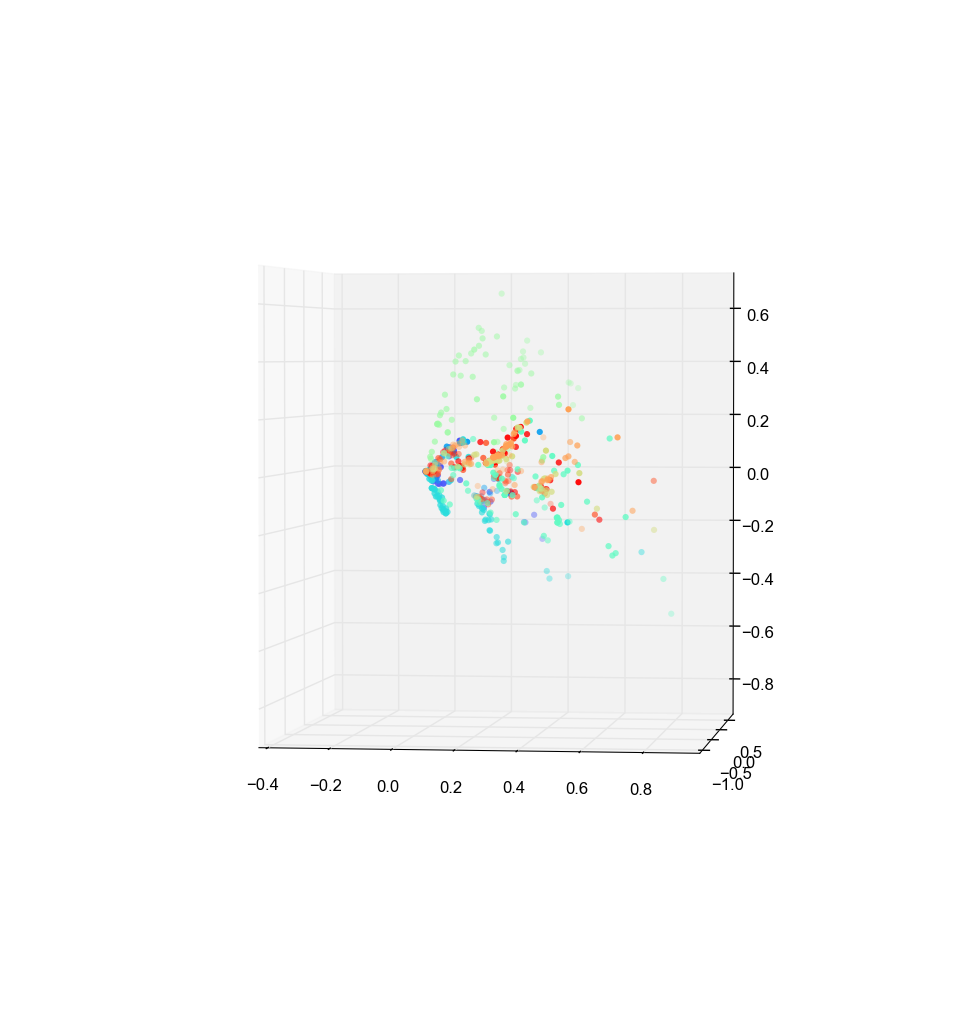
\includegraphics[width=\linewidth]{secciones/graficos/oja/1_train.png}
                \caption{Validacion}
                \label{fig: ej1_oja_3d_1_valid}
        \end{subfigure}
        \caption{Vista 1 en 3d de resultados de validación y entrenamiento}
        \label{fig: ej1_oja_3d_1}
\end{figure}

\begin{figure}[H]
        \begin{subfigure}[b]{0.5\textwidth}
                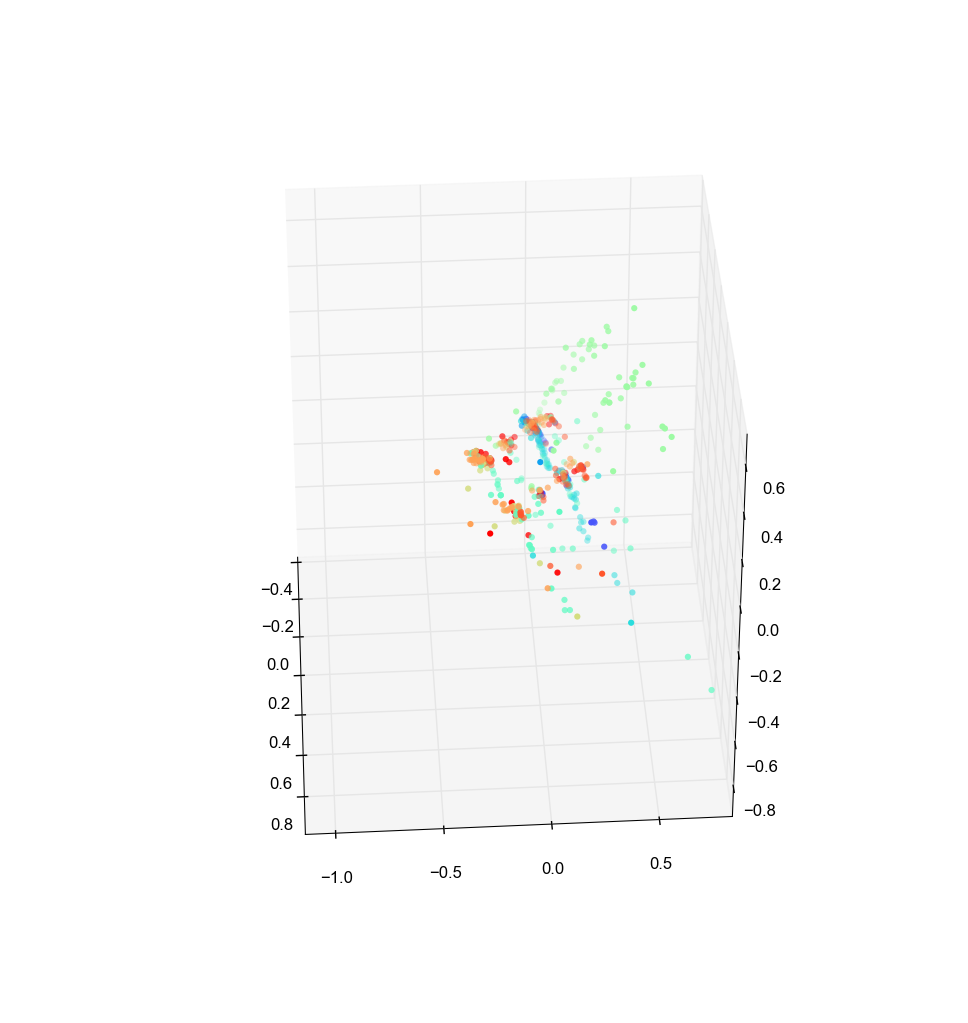
\includegraphics[width=\linewidth]{secciones/graficos/oja/2_train.png}
                \caption{Entrenamiento}
                \label{fig: ej1_oja_3d_2_train}
        \end{subfigure}%
        \begin{subfigure}[b]{0.5\textwidth}
                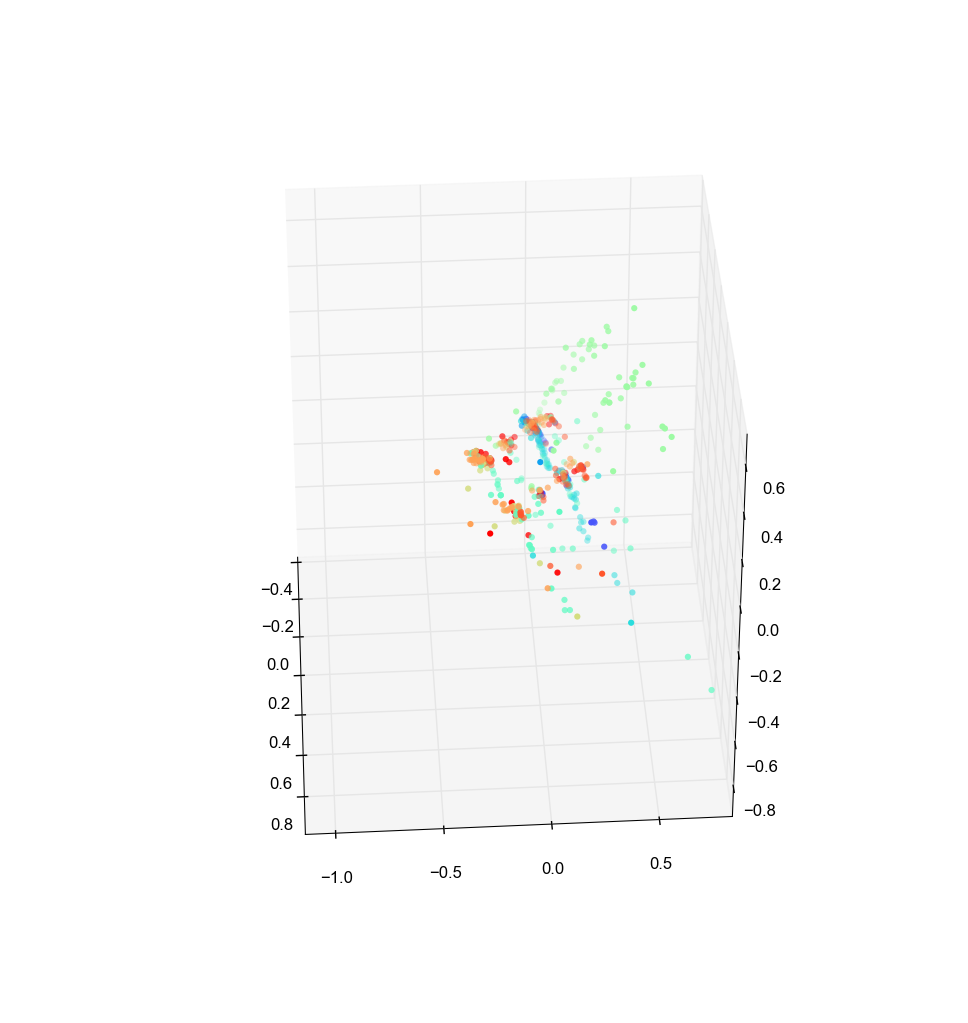
\includegraphics[width=\linewidth]{secciones/graficos/oja/2_train.png}
                \caption{Validacion}
                \label{fig: ej1_oja_3d_2_valid}
        \end{subfigure}
        \caption{Vista 2 en 3d de resultados de validación y entrenamiento}
        \label{fig: ej1_oja_3d_2}
\end{figure}


\par Se puede observar que la validación es consistente con la clasificación obtenida en la etapa de entrenamiento, dando cuenta de la validez del procedimiento realizado. También se puede observar en el gráfico claramente la separación entre dos de las categorías, la verde y azul, cosa que no ocurre para las categorías restantes. Para poder discriminar sobre estas últimas realizamos graficos 2d (figura \ref{fig: ej1_oja_ejes_train}), proyectando el gráfico 3d sobre tres planos distintos, tanto para los datos de entrenamiento \ref{fig: ej1_oja_ejes_train}  como para los de validación \ref{fig: ej1_oja_ejes_valid}.

\begin{figure}[H]
        \begin{subfigure}[b]{0.33\textwidth}
                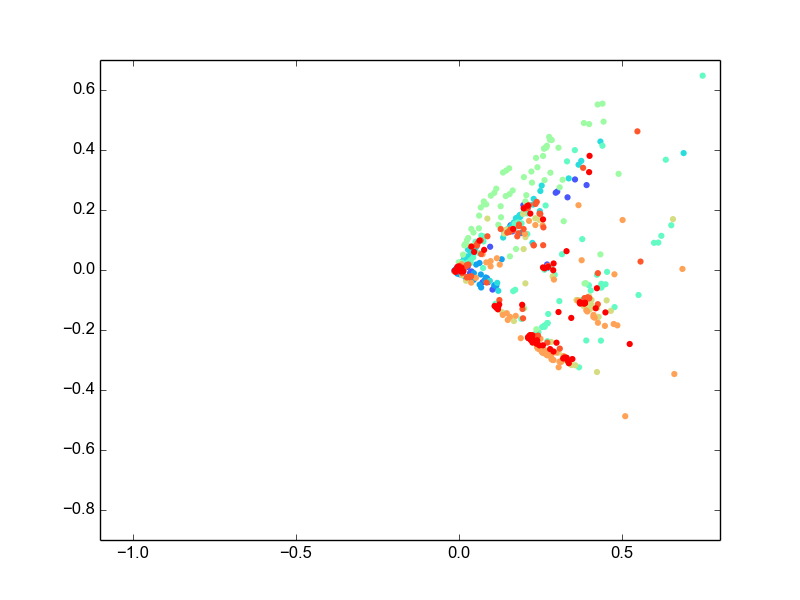
\includegraphics[width=\linewidth]{secciones/graficos/oja/eje1_train.png}
                \caption{Corte 1}
                \label{fig: ej1_oja_eje_1_train}
        \end{subfigure}
        \begin{subfigure}[b]{0.33\textwidth}
                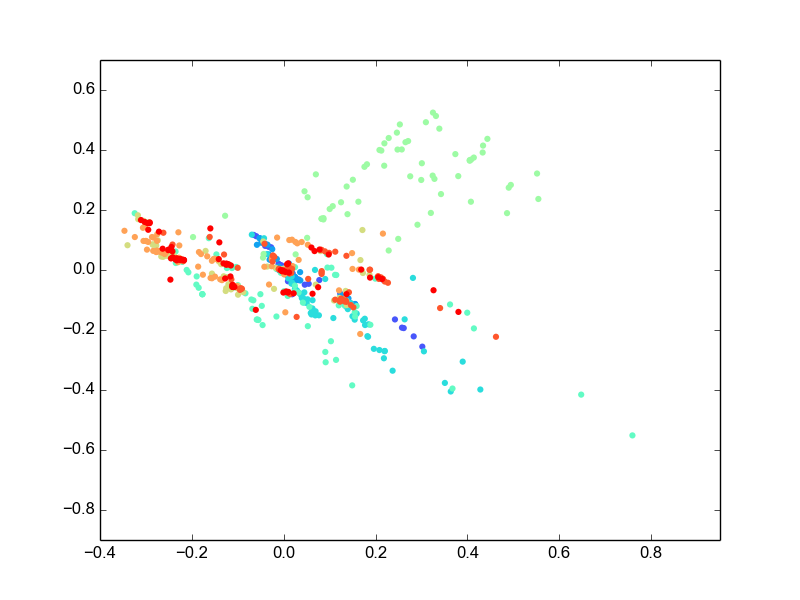
\includegraphics[width=\linewidth]{secciones/graficos/oja/eje2_train.png}
                \caption{Corte 2}
                \label{fig: ej1_oja_eje_2_train}
        \end{subfigure}
        \begin{subfigure}[b]{0.33\textwidth}
                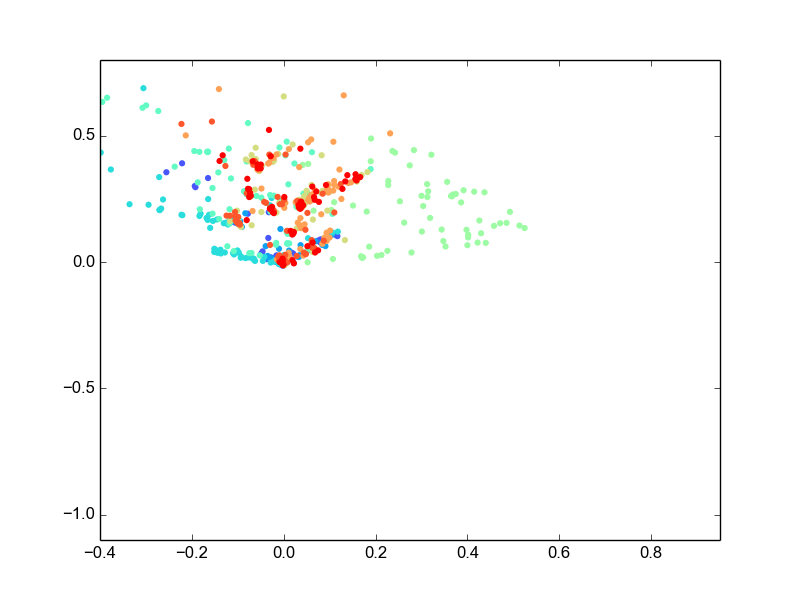
\includegraphics[width=\linewidth]{secciones/graficos/oja/eje3_train.png}
                \caption{Corte 3}
                \label{fig: ej1_oja_eje_3_train}
        \end{subfigure}
        \caption{Cortes del gráfico de los datos de entrenamiento}
        \label{fig: ej1_oja_ejes_train}
\end{figure}

\begin{figure}[H]
        \begin{subfigure}[b]{0.33\textwidth}
                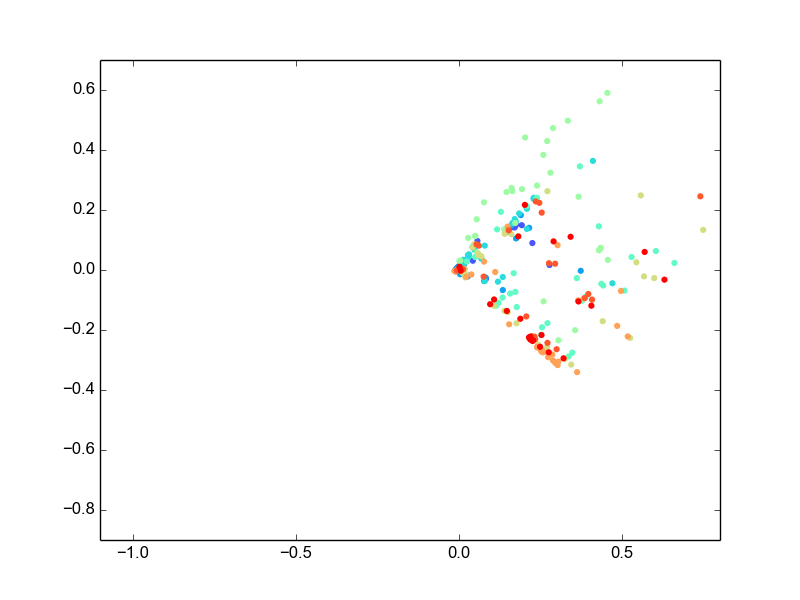
\includegraphics[width=\linewidth]{secciones/graficos/oja/eje1_valid.png}
                \caption{Corte 1}
                \label{fig: ej1_oja_eje_1_valid}
        \end{subfigure}
        \begin{subfigure}[b]{0.33\textwidth}
                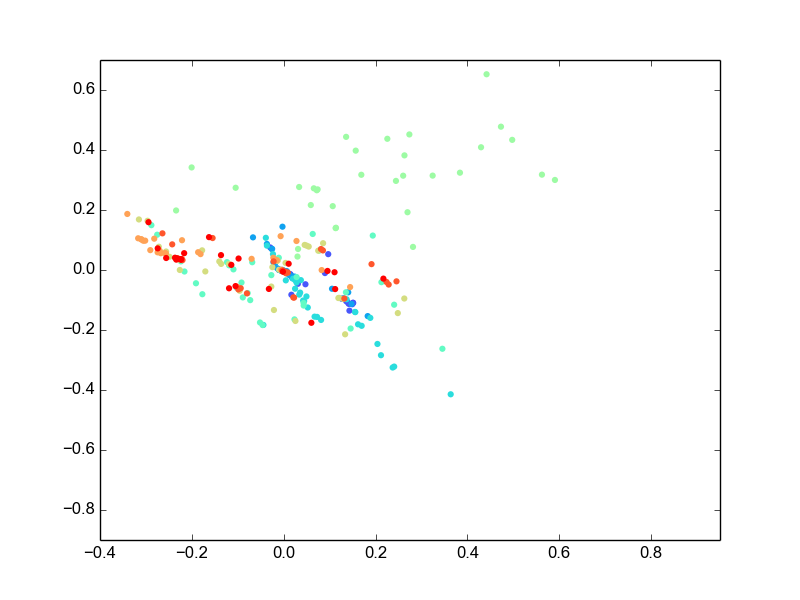
\includegraphics[width=\linewidth]{secciones/graficos/oja/eje2_valid.png}
                \caption{Corte 2}
                \label{fig: ej1_oja_eje_2_valid}
        \end{subfigure}
        \begin{subfigure}[b]{0.33\textwidth}
                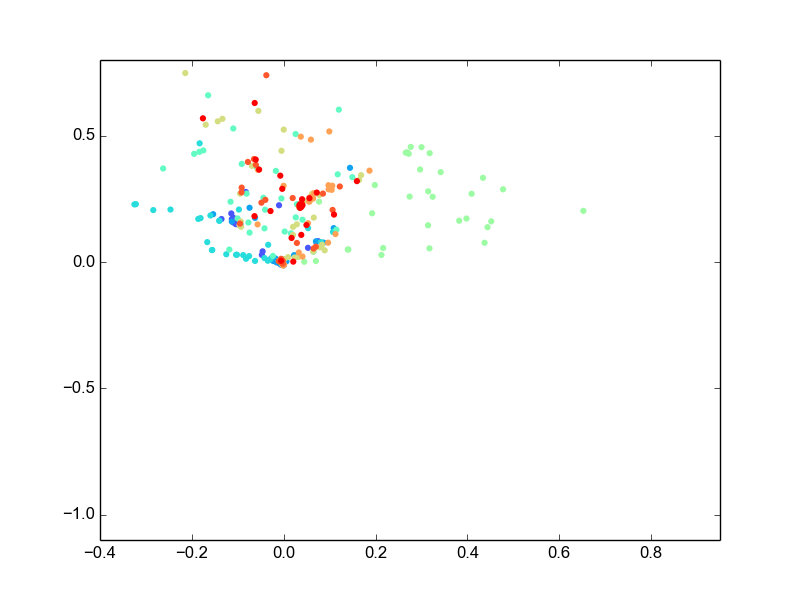
\includegraphics[width=\linewidth]{secciones/graficos/oja/eje3_valid.png}
                \caption{Corte 3}
                \label{fig: ej1_oja_eje_3_valid}
        \end{subfigure}
        \caption{Cortes del gráfico de los datos de validación}
        \label{fig: ej1_oja_ejes_valid}
\end{figure}


\par Estos gráficos permiten observar mejor las similitudes entre los resultados obtenidos con los datos de entrenamiento y los obtenidos con los datos de validación. No se distinguen resultados tan errado como para ser detectados a simple vista. Esto nos deja la impresión de que, a pesar de que las categorías no se separen y agrupen como esperábamos, la red generaliza bastante bien y es consistente en cuanto a la ubicación de las categorías.

\par A continuación realizamos un gráfico 3D para cada categoría en la etapa de entrenamiento, con la finalidad de poder observar su distribución individualmente, ya que en las figuras \ref{ej1_oja_ejes_train} se encuentran algo superpuestas. Los resultados se observan en las figuras \ref{fig: ej1_oja_categorias}.

\begin{figure}[H]
        \begin{subfigure}[b]{0.33\textwidth}
                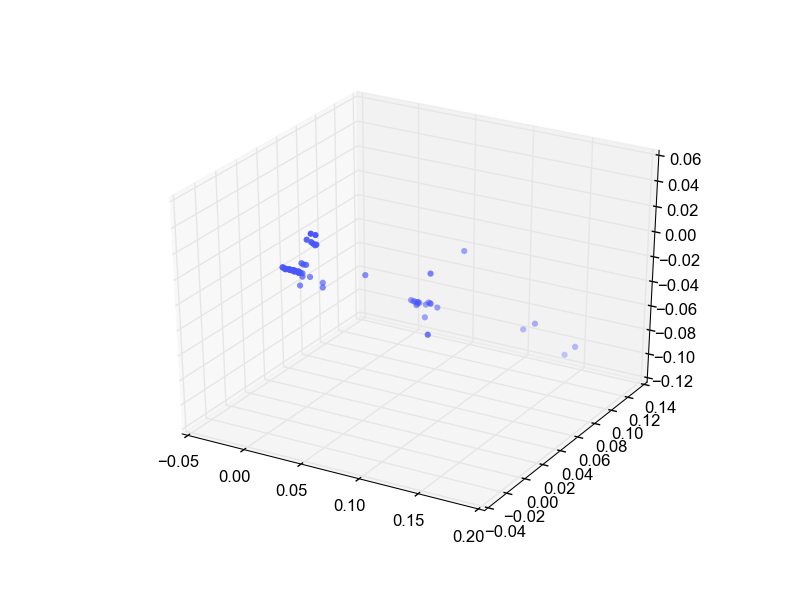
\includegraphics[width=\linewidth]{secciones/graficos/oja/categoria_1.png}
                \caption{Categoría 1}
                \label{fig: ej1_oja_categoria_1}
        \end{subfigure}
        \begin{subfigure}[b]{0.33\textwidth}
                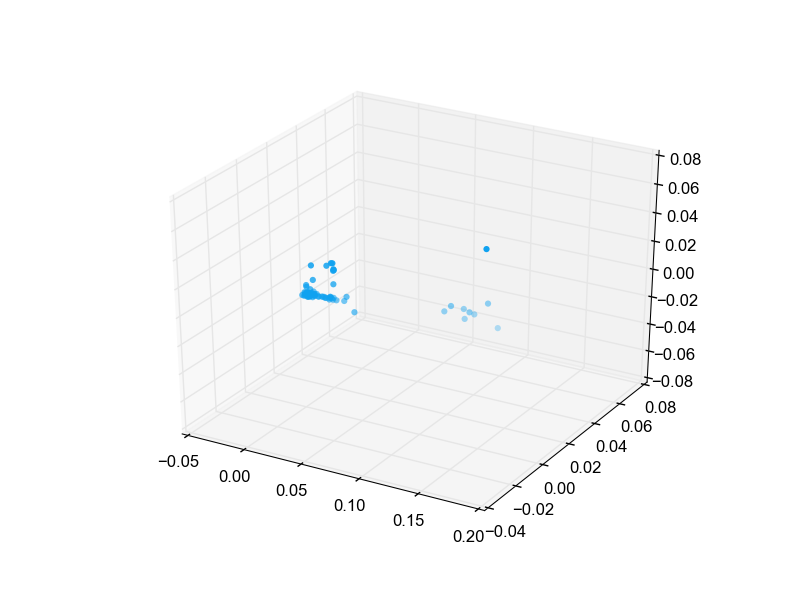
\includegraphics[width=\linewidth]{secciones/graficos/oja/categoria_2.png}
                \caption{Categoría 2}
                \label{fig: ej1_oja_categoria_2}
        \end{subfigure}
        \begin{subfigure}[b]{0.33\textwidth}
                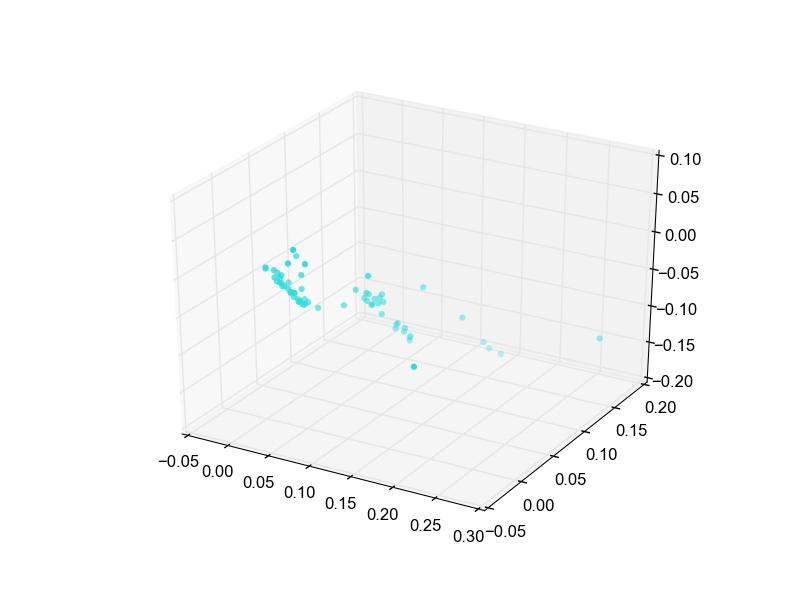
\includegraphics[width=\linewidth]{secciones/graficos/oja/categoria_3.png}
                \caption{Categoría 3}
                \label{fig: ej1_oja_categoria_4}
        \end{subfigure}
        \begin{subfigure}[b]{0.33\textwidth}
                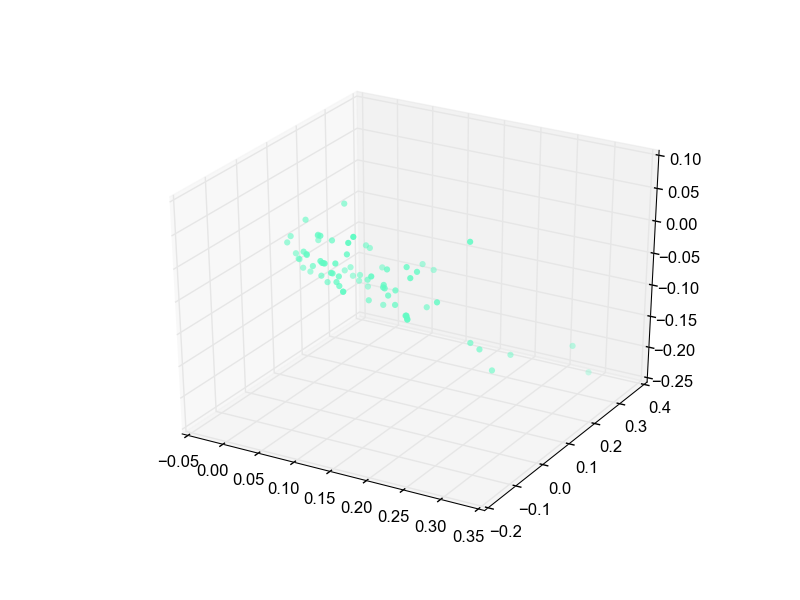
\includegraphics[width=\linewidth]{secciones/graficos/oja/categoria_4.png}
                \caption{Categoría 4}
                \label{fig: ej1_oja_categoria_4}
        \end{subfigure}
        \begin{subfigure}[b]{0.33\textwidth}
                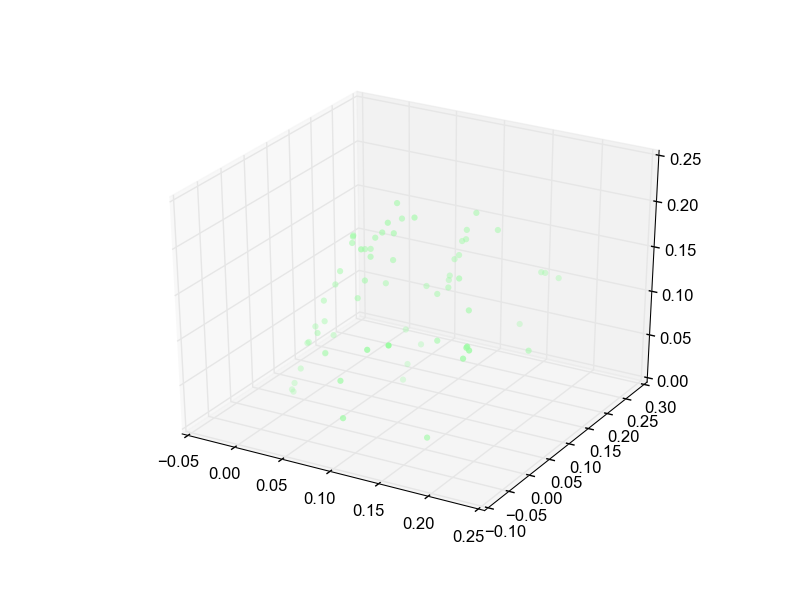
\includegraphics[width=\linewidth]{secciones/graficos/oja/categoria_5.png}
                \caption{Categoría 5}
                \label{fig: ej1_oja_categoria_5}
        \end{subfigure}
        \begin{subfigure}[b]{0.33\textwidth}
                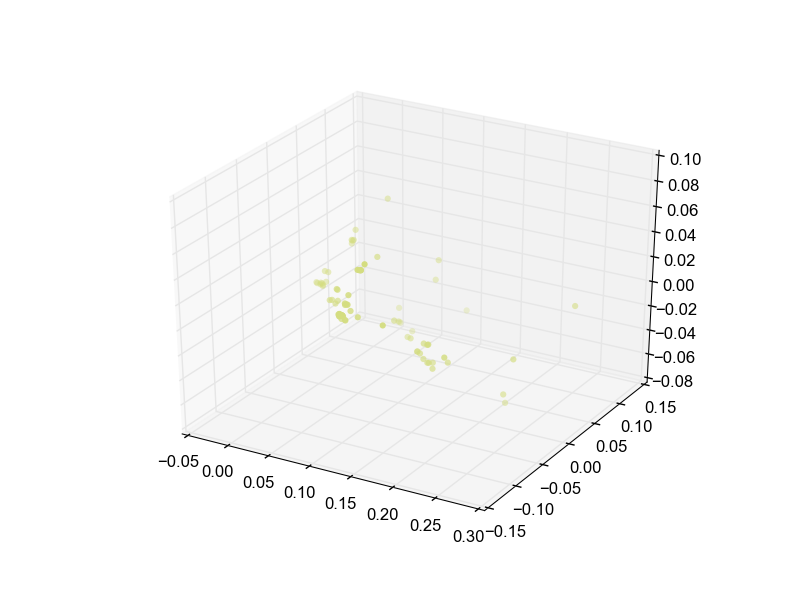
\includegraphics[width=\linewidth]{secciones/graficos/oja/categoria_6.png}
                \caption{Categoría 6}
                \label{fig: ej1_oja_categoria_6}
        \end{subfigure}
        \begin{subfigure}[b]{0.33\textwidth}
                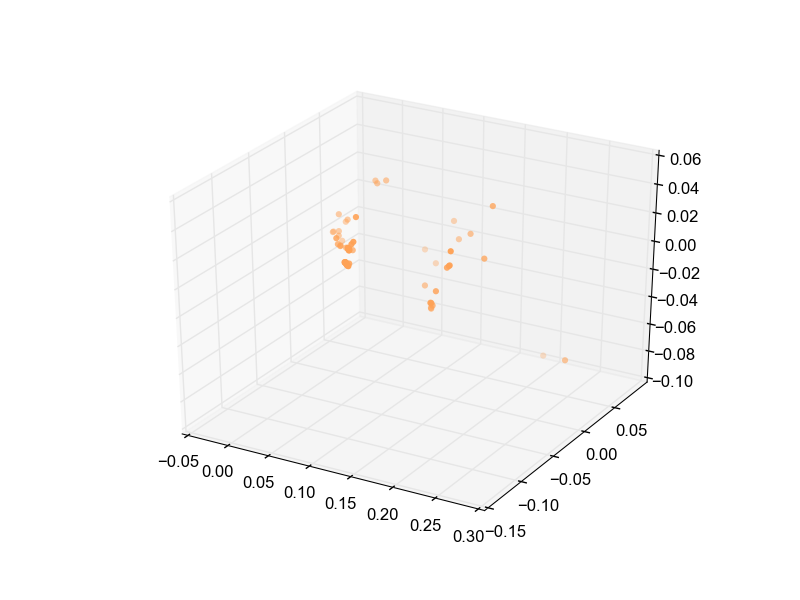
\includegraphics[width=\linewidth]{secciones/graficos/oja/categoria_7.png}
                \caption{Categoría 7}
                \label{fig: ej1_oja_categoria_7}
        \end{subfigure}
        \begin{subfigure}[b]{0.33\textwidth}
                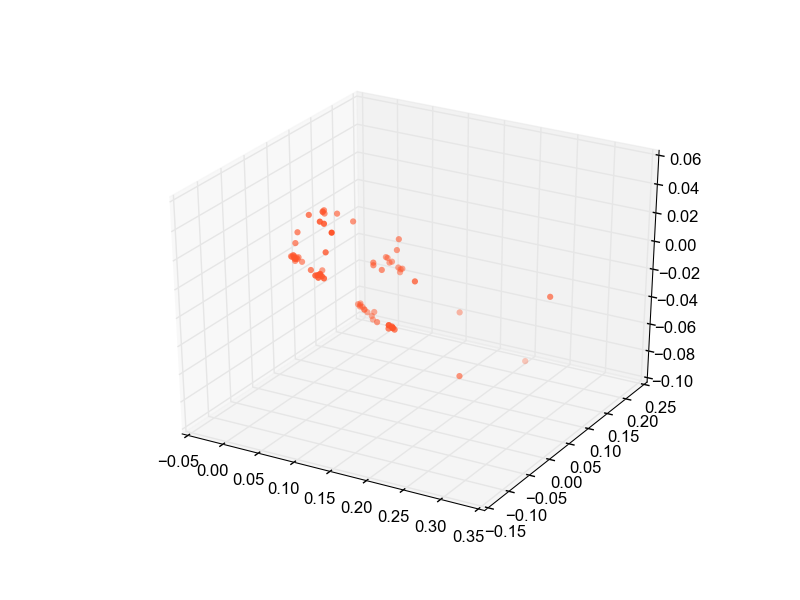
\includegraphics[width=\linewidth]{secciones/graficos/oja/categoria_8.png}
                \caption{Categoría 8}
                \label{fig: ej1_oja_categoria_8}
        \end{subfigure}
        \begin{subfigure}[b]{0.33\textwidth}
                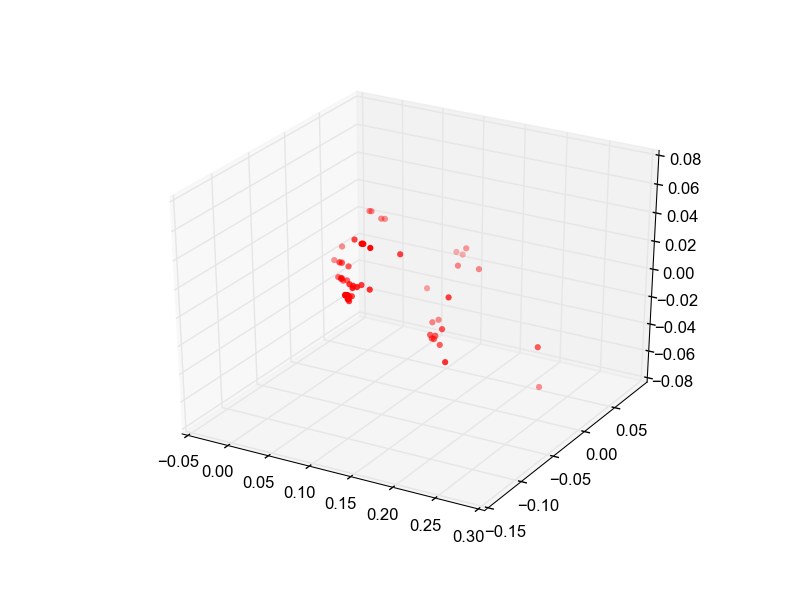
\includegraphics[width=\linewidth]{secciones/graficos/oja/categoria_9.png}
                \caption{Categoría 9}
                \label{fig: ej1_oja_categoria_9}
        \end{subfigure}
        \caption{Gráficos de resultados diferenciados por categoría}
        \label{fig: ej1_oja_categorias}
\end{figure}


\par Como observamos que algunas categorías se encontraban algo dispersas, calculamos la varianza promedio de los datos de cada categoría para ver si nos dan alguna señal de por qué puede estar ocurriendo esto. Los resultados se pueden observar en la siguiente figura \ref{fig: varianza_entrada}.

\begin{figure}[H]
        \centering
        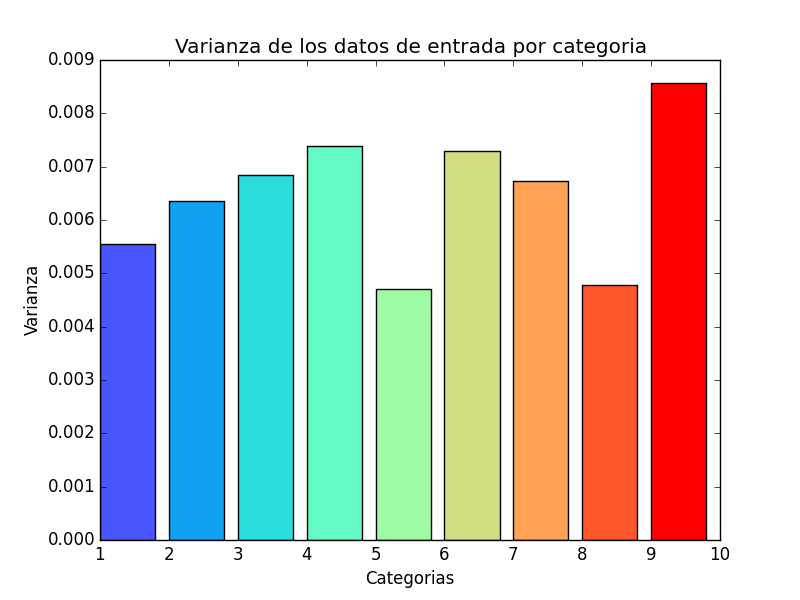
\includegraphics[width=0.8\linewidth]{secciones/graficos/varianza_entrada.png}
        \caption{Varianza de los datos de entrada por categoría}
        \label{fig: varianza_entrada}
\end{figure}

\par En la figura \ref{fig: ej1_oja_errores}, se puede observar como se satisface la condición de ortonormalidad, en función del número de época. Se aprecia que a partir de las 1000 épocas la norma se hace menor al 0.18 y continúa decreciendo fuértemente hasta valores por debajo de 0.02.


\begin{figure}[H]
        \begin{subfigure}[b]{0.5\textwidth}
                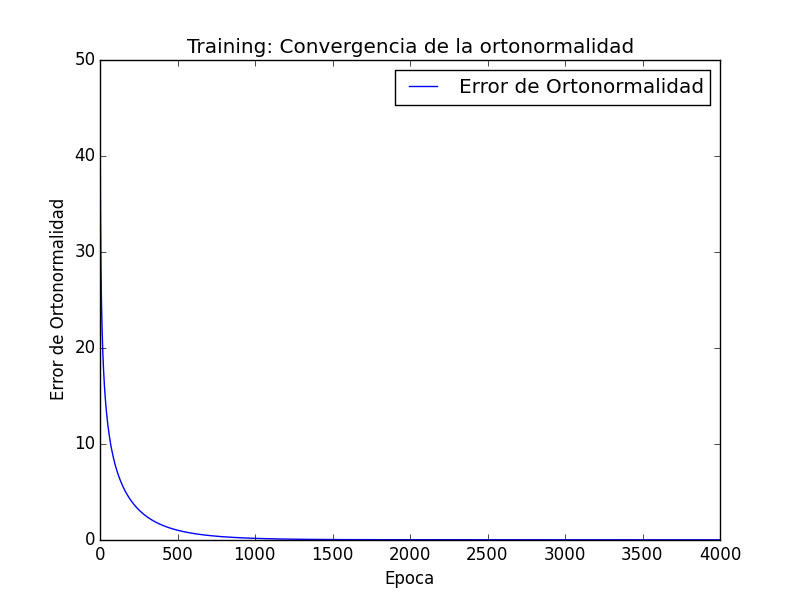
\includegraphics[width=\linewidth]{secciones/graficos/oja/error.png}
                \caption{Todas las épocas}
                \label{fig: ej1_oja_error}
        \end{subfigure}
        \begin{subfigure}[b]{0.5\textwidth}
                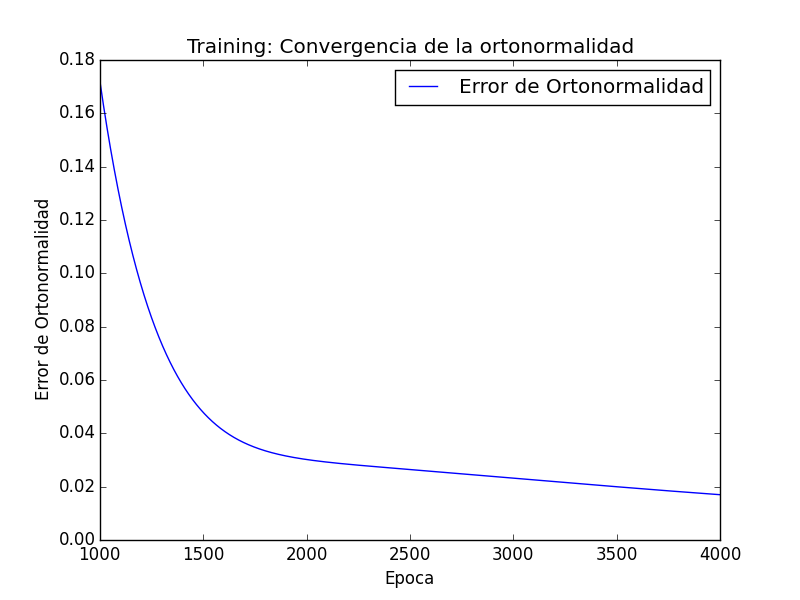
\includegraphics[width=\linewidth]{secciones/graficos/oja/error_zoom.png}
                \caption{A partir de la época 1000}
                \label{fig: ej1_oja_error_zoom}
        \end{subfigure}
        \caption{Ortonormalidad de la matriz de pesos en función de las épocas.}
        \label{fig: ej1_oja_errores}
\end{figure}


\subsubsection{Algoritmo de Sanger}

\par Se realizó una análisis similar al caso anterior, utilizando el mismo porcentaje de datos de entrenamiento - validación y el mismo coeficiente de aprendizaje adaptativo. En la figuras \ref{fig: ej1_sanger_3d_1} y \ref{fig: ej1_sanger_3d_2} se puede observar vistas 3d (componentes principales obtenidos por el algoritmo) de los datos de entrenamiento (figuras \ref{fig: ej1_sanger_3d_1_train}, \ref{fig: ej1_sanger_3d_2_train}) y validacion (figuras \ref{fig: ej1_sanger_3d_1_valid}, \ref{fig: ej1_sanger_3d_2_valid}). Al igual que en el caso anterior, obtenemos una buena clasificación sobre los datos de validación.

\begin{figure}[H]
        \begin{subfigure}[b]{0.5\textwidth}
                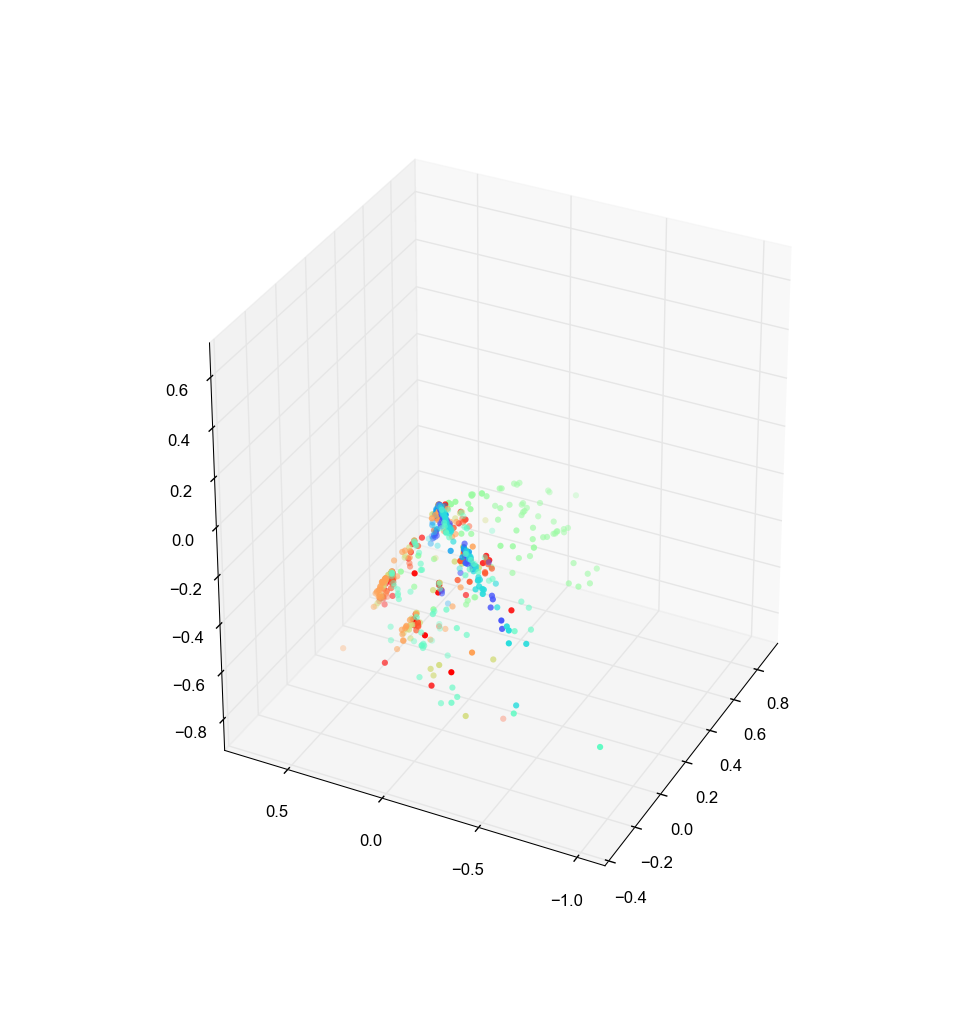
\includegraphics[width=\linewidth]{secciones/graficos/sanger/1_train.png}
                \caption{Entrenamiento}
                \label{fig: ej1_sanger_3d_1_train}
        \end{subfigure}%
        \begin{subfigure}[b]{0.5\textwidth}
                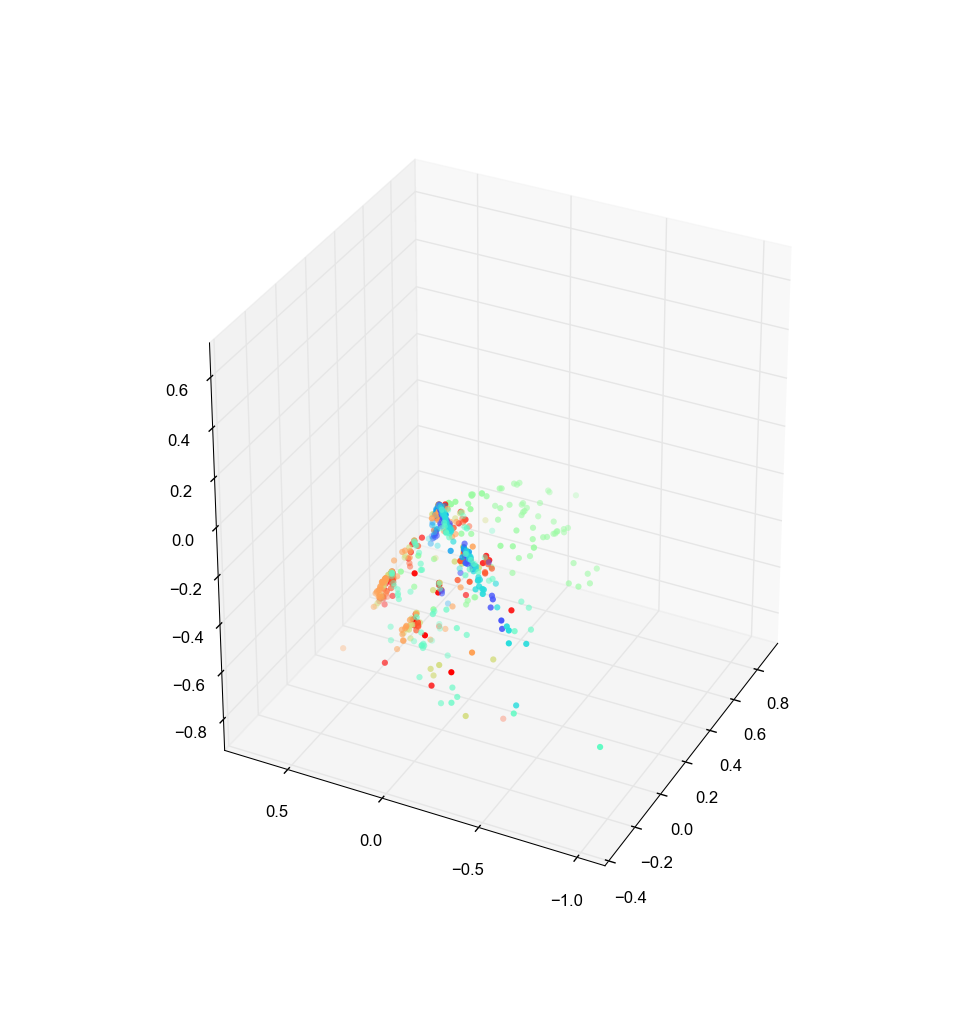
\includegraphics[width=\linewidth]{secciones/graficos/sanger/1_train.png}
                \caption{Validacion}
                \label{fig: ej1_sanger_3d_1_valid}
        \end{subfigure}
        \caption{Vista 1 en 3d de resultados de validación y entrenamiento}
        \label{fig: ej1_sanger_3d_1}
\end{figure}

\begin{figure}[H]
        \begin{subfigure}[b]{0.5\textwidth}
                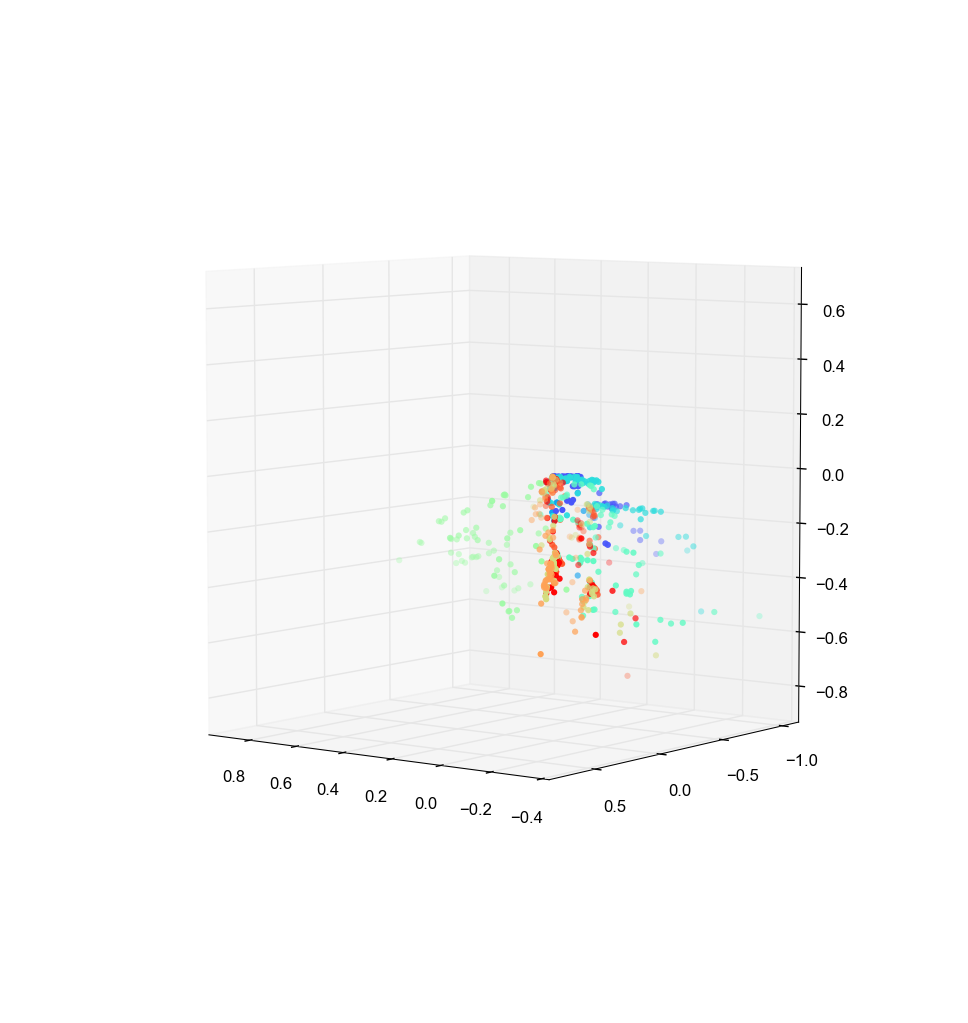
\includegraphics[width=\linewidth]{secciones/graficos/sanger/2_train.png}
                \caption{Entrenamiento}
                \label{fig: ej1_sanger_3d_2_train}
        \end{subfigure}
        \begin{subfigure}[b]{0.5\textwidth}
                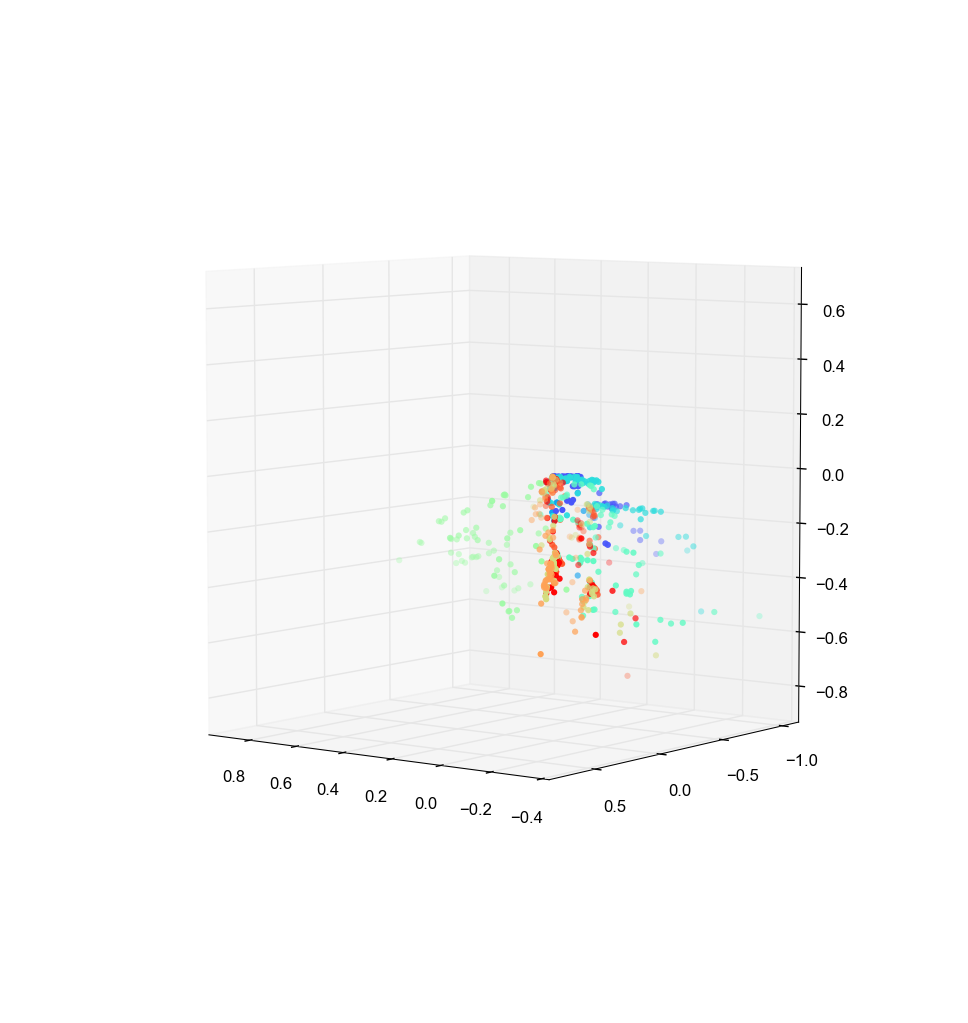
\includegraphics[width=\linewidth]{secciones/graficos/sanger/2_train.png}
                \caption{Validacion}
                \label{fig: ej1_sanger_3d_2_valid}
        \end{subfigure}
        \caption{Vista 2 en 3d de resultados de validación y entrenamiento}
        \label{fig: ej1_sanger_3d_2}
\end{figure}

\par proyectando estos gráficos 3d sobre distintos planos, obtenemos las siguientes figuras, tanto para entrenamiento figuras \ref{fig: ej1_sanger_ejes_train} como para validación figura \ref{fig: ej1_sanger_ejes_valid}

\begin{figure}[H]
        \begin{subfigure}[b]{0.33\textwidth}
                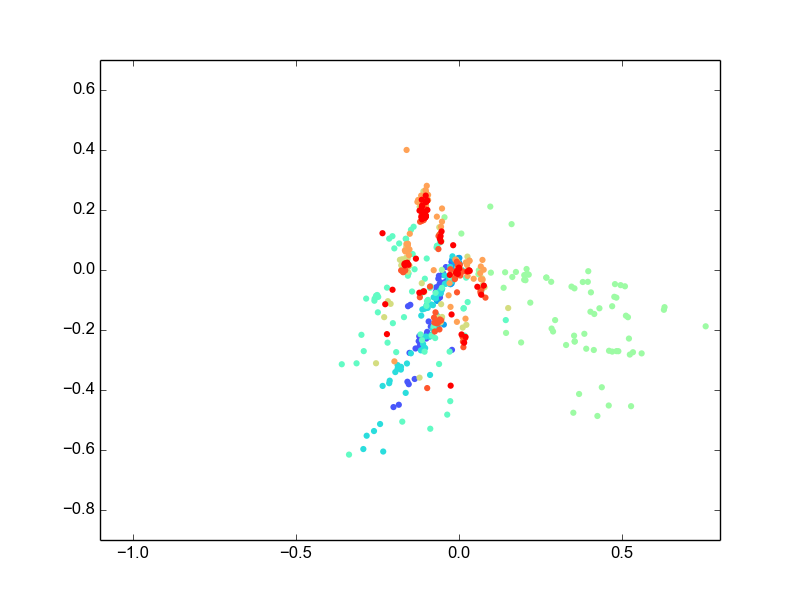
\includegraphics[width=\linewidth]{secciones/graficos/sanger/eje1_train.png}
                \caption{Corte 1}
                \label{fig: ej1_sanger_eje_1_train}
        \end{subfigure}
        \begin{subfigure}[b]{0.33\textwidth}
                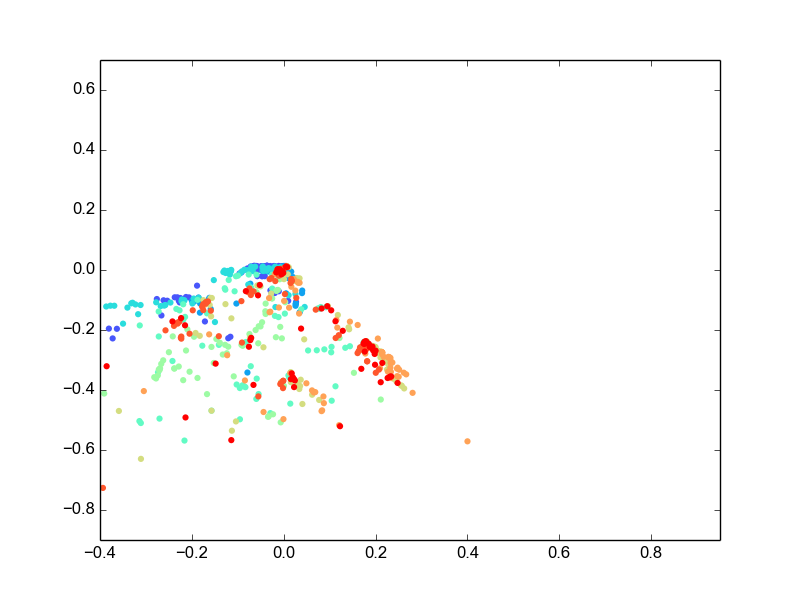
\includegraphics[width=\linewidth]{secciones/graficos/sanger/eje2_train.png}
                \caption{Corte 2}
                \label{fig: ej1_sanger_eje_2_train}
        \end{subfigure}
        \begin{subfigure}[b]{0.33\textwidth}
                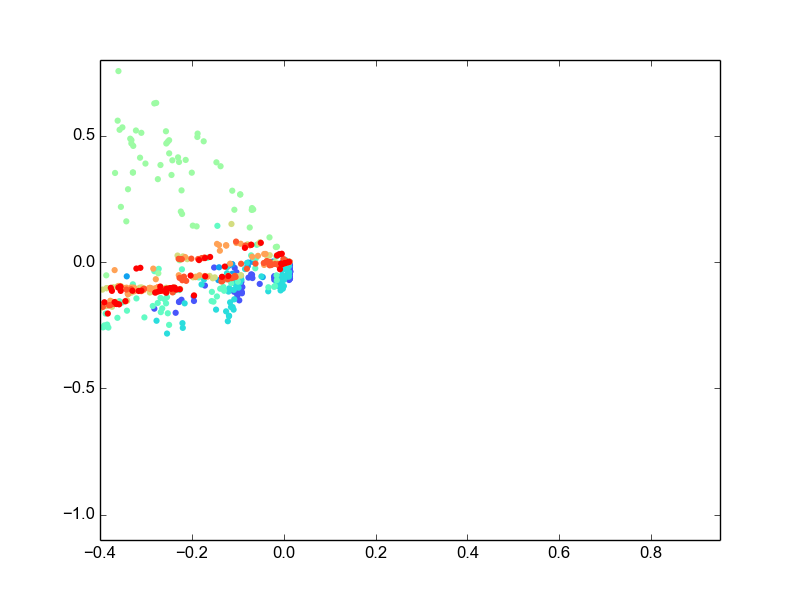
\includegraphics[width=\linewidth]{secciones/graficos/sanger/eje3_train.png}
                \caption{Corte 3}
                \label{fig: ej1_sanger_eje_3_train}
        \end{subfigure}
        \caption{Cortes del gráfico de los datos de entrenamiento}
        \label{fig: ej1_sanger_ejes_train}
\end{figure}

\begin{figure}[H]
        \begin{subfigure}[b]{0.33\textwidth}
                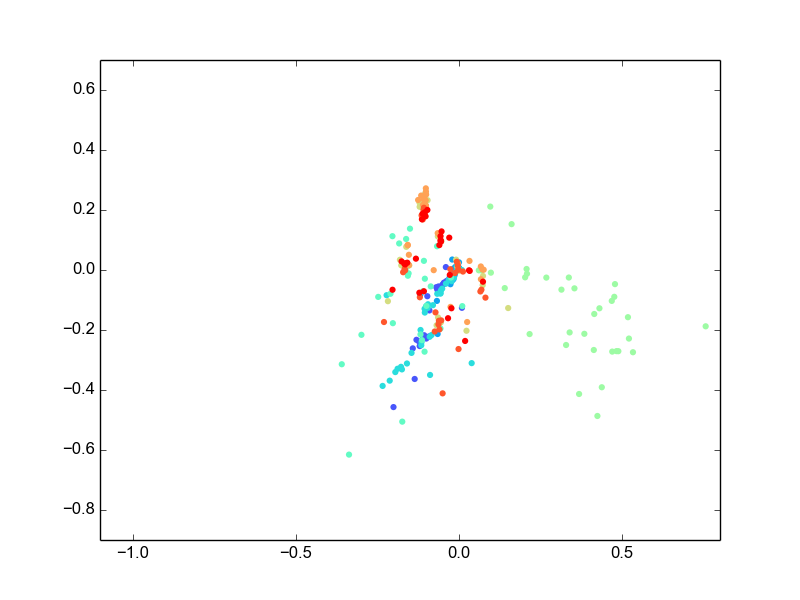
\includegraphics[width=\linewidth]{secciones/graficos/sanger/eje1_valid.png}
                \caption{Corte 1}
                \label{fig: ej1_sanger_eje_1_valid}
        \end{subfigure}
        \begin{subfigure}[b]{0.33\textwidth}
                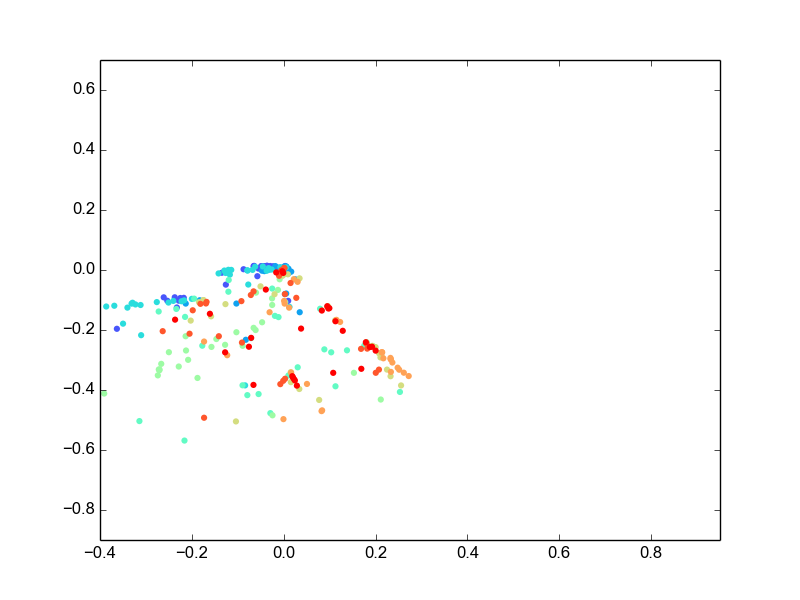
\includegraphics[width=\linewidth]{secciones/graficos/sanger/eje2_valid.png}
                \caption{Corte 2}
                \label{fig: ej1_sanger_eje_2_valid}
        \end{subfigure}
        \begin{subfigure}[b]{0.33\textwidth}
                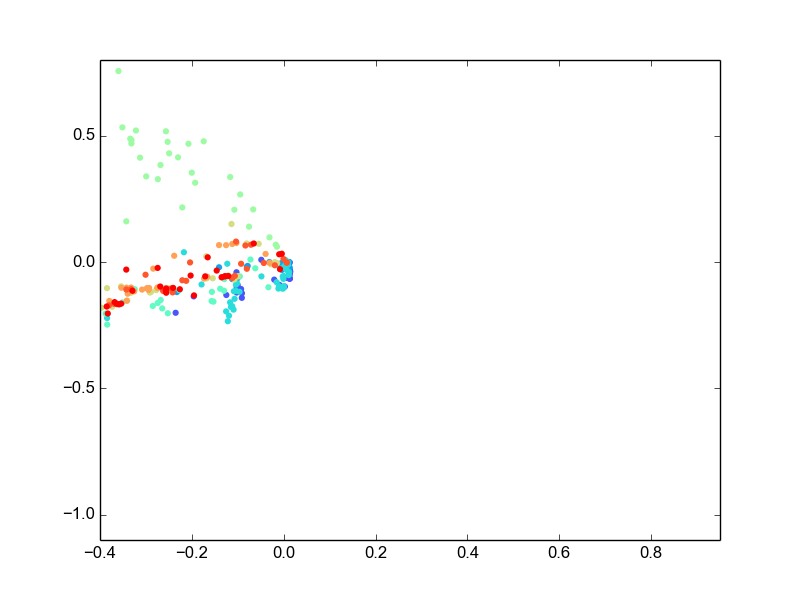
\includegraphics[width=\linewidth]{secciones/graficos/sanger/eje3_valid.png}
                \caption{Corte 3}
                \label{fig: ej1_sanger_eje_3_valid}
        \end{subfigure}
        \caption{Cortes del gráfico de los datos de validación}
        \label{fig: ej1_sanger_ejes_valid}
\end{figure}


\par A continuación podemos observar los resultados de entrenamiento en gráficos 3d para las distintas categorías, con el fin de observar más claramente como se distribuyen los mismos (figuras \ref{fig: ej1_sanger_categorias}). 

\begin{figure}[H]
        \begin{subfigure}[b]{0.33\textwidth}
                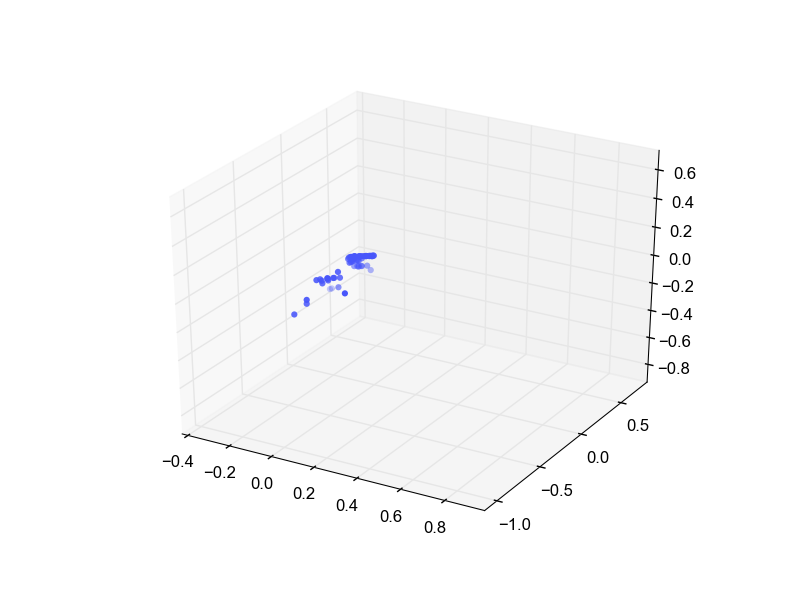
\includegraphics[width=\linewidth]{secciones/graficos/sanger/categoria_1.png}
                \caption{Categoría 1}
                \label{fig: ej1_sanger_categoria_1}
        \end{subfigure}
        \begin{subfigure}[b]{0.33\textwidth}
                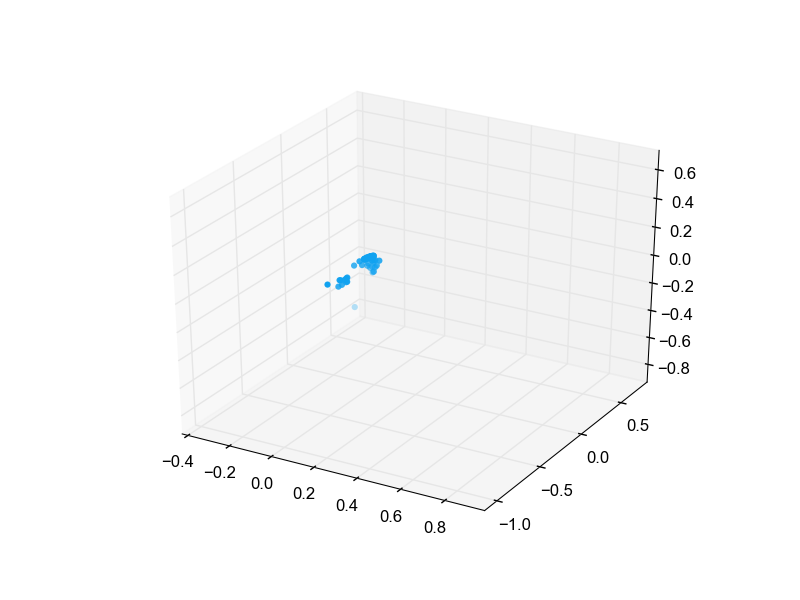
\includegraphics[width=\linewidth]{secciones/graficos/sanger/categoria_2.png}
                \caption{Categoría 2}
                \label{fig: ej1_sanger_categoria_2}
        \end{subfigure}
        \begin{subfigure}[b]{0.33\textwidth}
                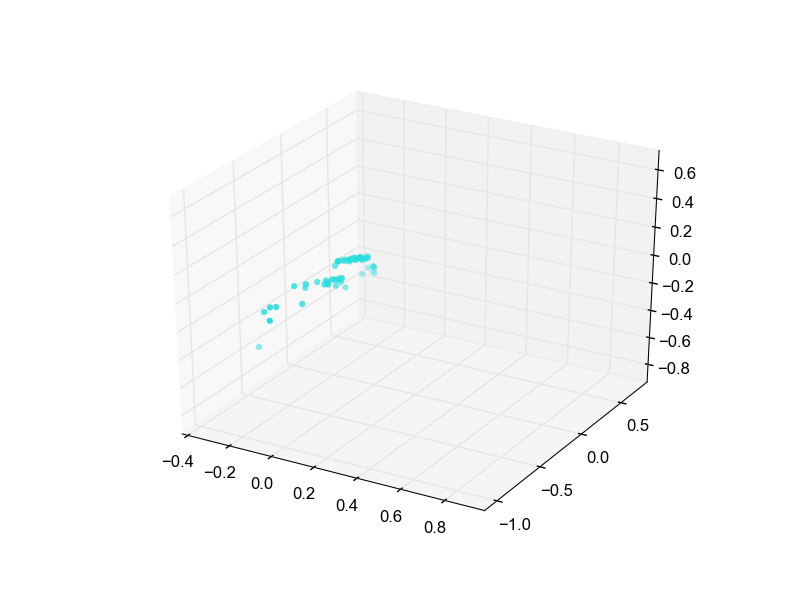
\includegraphics[width=\linewidth]{secciones/graficos/sanger/categoria_3.png}
                \caption{Categoría 3}
                \label{fig: ej1_sanger_categoria_4}
        \end{subfigure}
        \begin{subfigure}[b]{0.33\textwidth}
                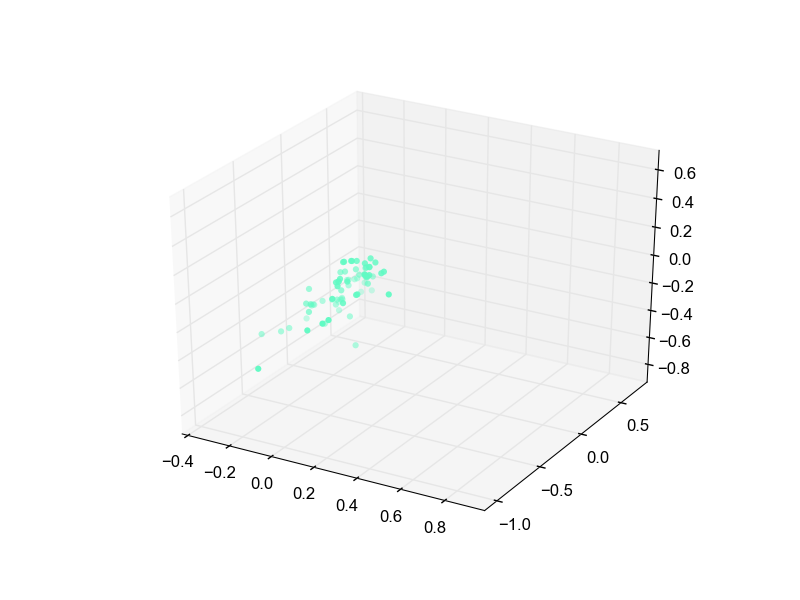
\includegraphics[width=\linewidth]{secciones/graficos/sanger/categoria_4.png}
                \caption{Categoría 4}
                \label{fig: ej1_sanger_categoria_4}
        \end{subfigure}
        \begin{subfigure}[b]{0.33\textwidth}
                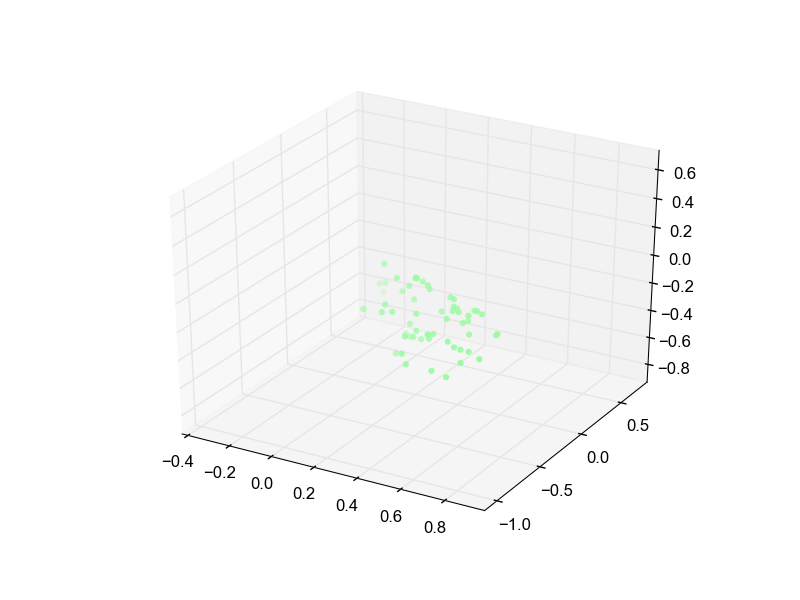
\includegraphics[width=\linewidth]{secciones/graficos/sanger/categoria_5.png}
                \caption{Categoría 5}
                \label{fig: ej1_sanger_categoria_5}
        \end{subfigure}
        \begin{subfigure}[b]{0.33\textwidth}
                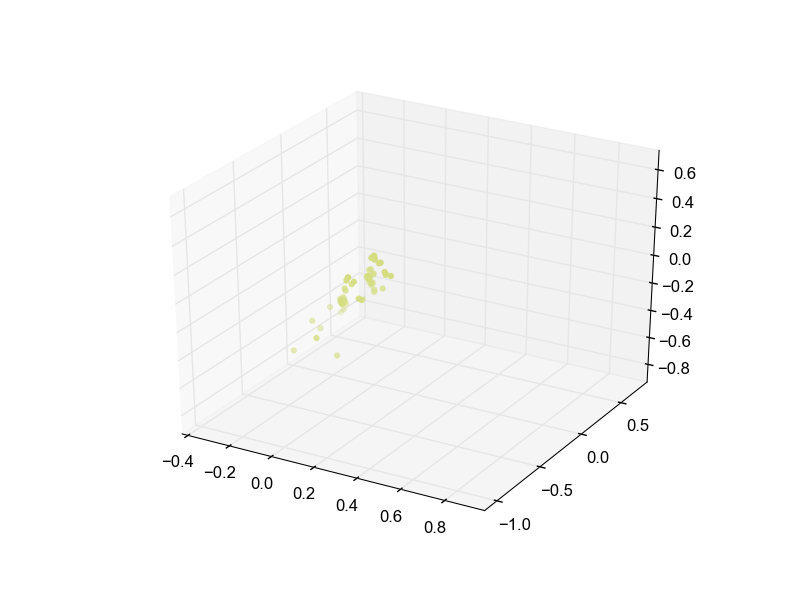
\includegraphics[width=\linewidth]{secciones/graficos/sanger/categoria_6.png}
                \caption{Categoría 6}
                \label{fig: ej1_sanger_categoria_6}
        \end{subfigure}
        \begin{subfigure}[b]{0.33\textwidth}
                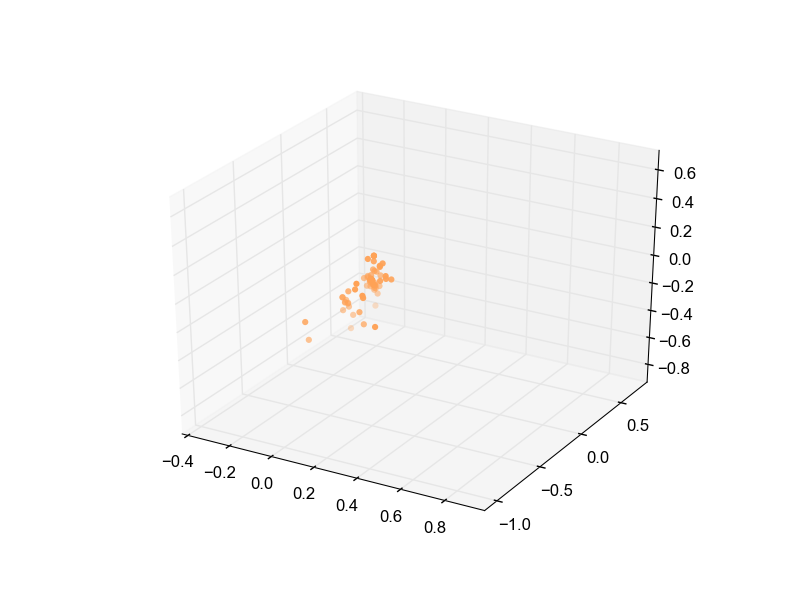
\includegraphics[width=\linewidth]{secciones/graficos/sanger/categoria_7.png}
                \caption{Categoría 7}
                \label{fig: ej1_sanger_categoria_7}
        \end{subfigure}
        \begin{subfigure}[b]{0.33\textwidth}
                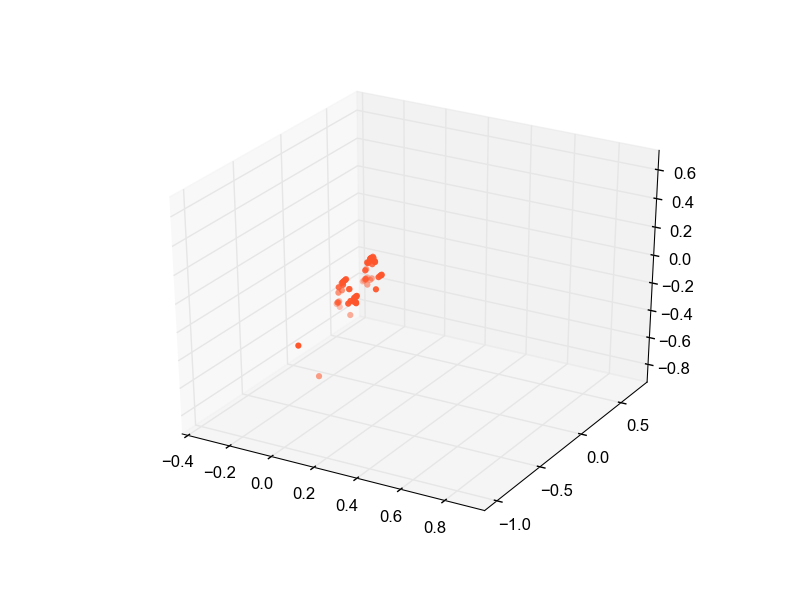
\includegraphics[width=\linewidth]{secciones/graficos/sanger/categoria_8.png}
                \caption{Categoría 8}
                \label{fig: ej1_sanger_categoria_8}
        \end{subfigure}
        \begin{subfigure}[b]{0.33\textwidth}
                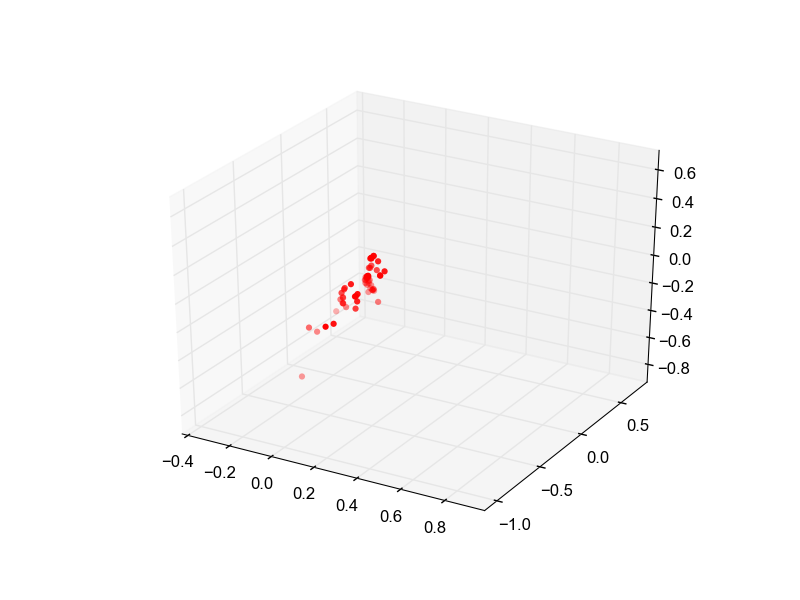
\includegraphics[width=\linewidth]{secciones/graficos/sanger/categoria_9.png}
                \caption{Categoría 9}
                \label{fig: ej1_sanger_categoria_9}
        \end{subfigure}
        \label{fig: ej1_sanger_categorias}
\end{figure}


\par Cabe destacar que los datos de entrada son los mismos tanto para Oja como para Sanger. Por lo que la varianza observada en la figura \ref{fig: varianza_entrada} también aplica para esta regla de aprendizaje y debemos tenerla en cuenta a la hora de comprender la dispersión de los datos de las categorías en los gráficos obtenidos.


\par En las figuras \ref{fig: ej1_sanger_errores}, se puede observar como se satisface la condición de ortonormalidad, en función del número de época. Se aprecia que a partir de las 1000 épocas la norma se hace menor al 0.0004, un valor muy bajo, y continúa decreciendo.

\begin{figure}[H]
        \begin{subfigure}[b]{0.5\textwidth}
                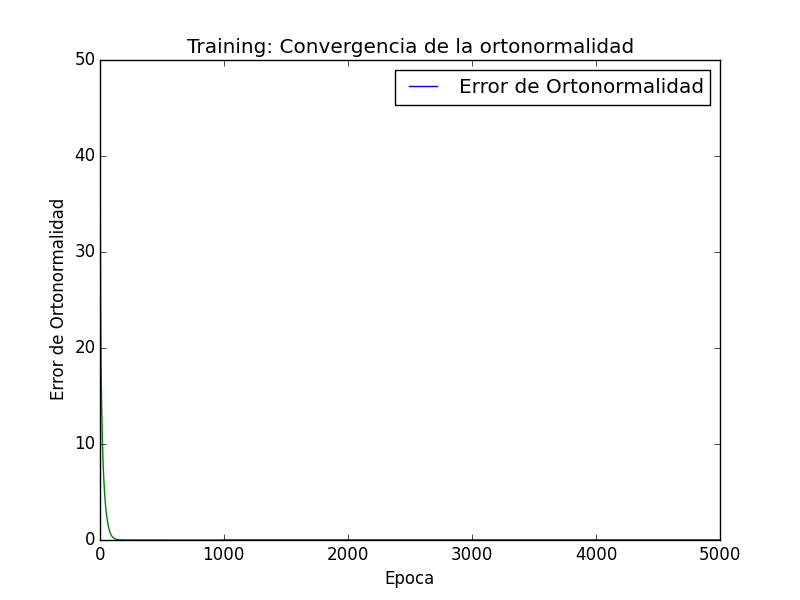
\includegraphics[width=\linewidth]{secciones/graficos/sanger/error.png}
                \caption{Todas las épocas}
                \label{fig: ej1_sanger_error}
        \end{subfigure}
        \begin{subfigure}[b]{0.5\textwidth}
                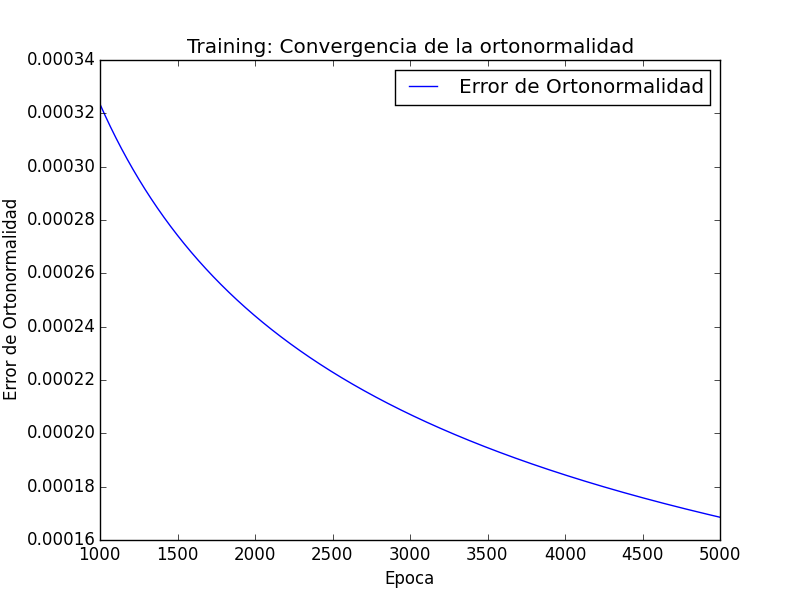
\includegraphics[width=\linewidth]{secciones/graficos/sanger/error_zoom.png}
                \caption{A partir de la época 1000}
                \label{fig: ej1_sanger_error_zoom}
        \end{subfigure}
        \caption{Ortonormalidad de la matriz de pesos en función de las épocas.}
        \label{fig: ej1_sanger_errores}
\end{figure}

\subsection{Conclusiones}

\par Se implementaron dos algoritmos para reducir la dimensionalidad del set de datos de entrada. Tanto el algoritmo de Sanger como el de Oja nos permiten obtener una clasificación que es consistente con los datos de validación. La diferencia entre los algortimos radica en que el de sanger nos permite obtener las componente principales, mientras que el de oja nos da un subespacio generado por estos, pero no nos da explicitamente las direcciones. Contrario a lo esperado, no pudimos visualizar esta diferencia. 
